% --- IMPORTS ---
\documentclass[leqno]{article}
\usepackage{graphicx}
\usepackage{dsfont}
\usepackage{mathtools}
\usepackage{amssymb}
\usepackage{amsmath}
\usepackage{amsthm}
\usepackage{float}
\usepackage{ragged2e}
\usepackage{tensor}
\usepackage{fancyhdr}
\usepackage{empheq}
\usepackage[most]{tcolorbox}
\usepackage{enumitem}
\usepackage{dirtytalk}
\usepackage{marginnote}
\usepackage{microtype}
\usepackage[
  a4paper,
  left=0.8in,
  right=1in,
  top=1in,
  bottom=0.5in,
  headheight=14pt,
  headsep=0.4in
]{geometry}
\setlength{\parindent}{0cm}
% --- TikZ Packages ---
\usepackage{pgfplots}
\pgfplotsset{compat=1.18}
\usepgfplotslibrary{fillbetween, polar}
\usetikzlibrary{calc, positioning}
\usetikzlibrary{angles, quotes}
\usetikzlibrary{arrows.meta}
\usetikzlibrary{decorations.pathreplacing, decorations.markings}
\usetikzlibrary{patterns}
\usetikzlibrary{intersections}
% --- URL Packages ---
\usepackage[colorlinks=true,linkcolor=red,citecolor=magenta,urlcolor=black]{hyperref}%
\urlstyle{same}
% --- END OF IMPORTS ---

% --- CUSTOM COMMANDS ---
\RenewDocumentCommand{\marks}{o m}{%
  \IfValueTF{#1}%
    {\marginnote{\raggedright\textbf{[#2]}}[#1]}%
    {\marginnote{\raggedright\textbf{[#2]}}}%
}
\newcommand{\vspacerule}[2]{%
  \par\vspace*{#1}%
  \noindent\hrulefill\par
  \vspace*{#2}%
}
\definecolor{scarlet}{RGB}{205, 40, 75}
\newcommand{\questionitem}{%
  \item\phantomsection
  \addcontentsline{toc}{section}{Question \number\value{enumi}}%
}
\renewcommand{\contentsname}{Questions}
% --- END OF CUSTOM COMMANDS ---

% --- HEADER CONFIG ---
\pagestyle{fancy}
\fancyhead{}
\fancyfoot{}
\renewcommand{\headrulewidth}{0.9pt}
\lhead{Collisions in 1 Dimension}
\chead{}
\rhead{\href{https://danieljsmith.org}{danieljsmith.org}}
% --- END OF HEADER CONFIG ---

\begin{document}
\vspace*{20pt}
\tableofcontents
\newpage
\begin{enumerate}[
  label=\textbf{\arabic*.},
  leftmargin=*,
  topsep=0pt,
  partopsep=0pt,
  parsep=0pt
]


% ---- Question 1 ----
\questionitem
% [Source: _QBT__Collisions_in_1_Dimension, Q1]

A particle $A$ of mass $2m$ and a particle $B$ of mass $3m$ are moving along the same straight line on a smooth horizontal surface. The particles are moving in opposite directions towards each other when they collide directly. \\

Immediately before the collision, the speed of $A$ is $4u$ and the speed of $B$ is $ku$. \\
Immediately after the collision, $A$ rebounds with speed $v$ and the speed of $B$ is $v$. \\

The magnitude of the impulse received by $A$ in the collision is $12mu$. \\
\begin{enumerate}[label=\textbf{(\alph*)}]
  \item Find $v$ in terms of $u$ only. \marks{3} \\
  \item Find the two possible values of $k$. \marks{5} \\
\end{enumerate}

\newpage

% ---- Question 2 ----
\questionitem
% [Source: _QBT__Collisions_in_1_Dimension, Q2]

\begin{figure}[H]
    \centering
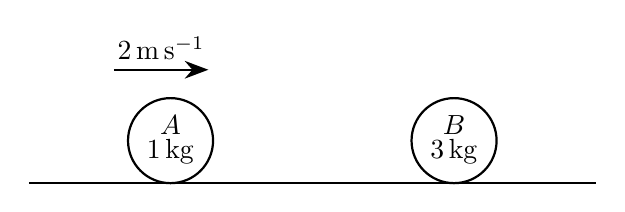
\begin{tikzpicture}[scale=1.2]
\def\rad{0.45}
\def\surf{6}
\def\arr{1.0}
\coordinate (L) at (0,0);
\coordinate (R) at (\surf,0);
\coordinate (A) at (1.5,\rad);
\coordinate (B) at (4.5,\rad);
\coordinate (Va) at ($(A)+(-0.6,0.75)$);
\draw[thick] (L) -- (R);
\draw[thick] (A) circle (\rad);
\draw[thick] (B) circle (\rad);
\draw[-{Stealth[length=3mm]}, thick] (Va) -- ++(\arr,0) node[midway, above] {$2\,\mathrm{m}\,\mathrm{s}^{-1}$};
\node at ($(A)+(0,0.16)$) {$A$};
\node at ($(A)+(0,-0.12)$) {$1\,\mathrm{kg}$};
\node at ($(B)+(0,0.16)$) {$B$};
\node at ($(B)+(0,-0.12)$) {$3\,\mathrm{kg}$};
\end{tikzpicture}
\end{figure}


The first diagram shows two spheres, $A$ and $B$, of equal radii on a smooth horizontal surface. Their masses are $1\,\mathrm{kg}$ and $3\,\mathrm{kg}$ respectively. \\

Take motion from left to right in each diagram to be positive. \\

Initially, sphere $A$ travels at speed $2\,\mathrm{m}\,\mathrm{s}^{-1}$ towards $B$, which is at rest. The spheres collide and the coefficient of restitution between $A$ and $B$ is $e$. \\
\begin{enumerate}[label=\textbf{(\alph*)}]
  \item Show that, after the collision, the velocity of $A$ is $\dfrac{1}{2}(1-3e)\,\mathrm{m}\,\mathrm{s}^{-1}$, and find an expression for the velocity of $B$ in terms of $e$. \marks{4} \\
  \item During the collision, the kinetic energy of the system decreases by $48\%$. Determine the value of $e$. \marks{3} \\
  \item Explain why the assumption that $A$ and $B$ have equal radii was needed in part (a). \marks{1} \\
\end{enumerate}


\begin{figure}[H]
    \centering
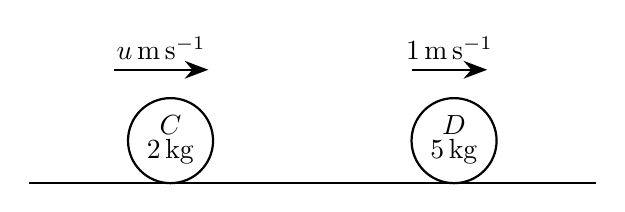
\begin{tikzpicture}[scale=1.2]
\def\rad{0.45}
\def\surf{6}
\def\arrc{1.0}
\def\arrd{0.8}
\coordinate (L) at (0,0);
\coordinate (R) at (\surf,0);
\coordinate (C) at (1.5,\rad);
\coordinate (D) at (4.5,\rad);
\coordinate (Vc) at ($(C)+(-0.6,0.75)$);
\coordinate (Vd) at ($(D)+(-0.45,0.75)$);
\draw[thick] (L) -- (R);
\draw[thick] (C) circle (\rad);
\draw[thick] (D) circle (\rad);
\draw[-{Stealth[length=3mm]}, thick] (Vc) -- ++(\arrc,0) node[midway, above] {$u\,\mathrm{m}\,\mathrm{s}^{-1}$};
\draw[-{Stealth[length=3mm]}, thick] (Vd) -- ++(\arrd,0) node[midway, above] {$1\,\mathrm{m}\,\mathrm{s}^{-1}$};
\node at ($(C)+(0,0.16)$) {$C$};
\node at ($(C)+(0,-0.12)$) {$2\,\mathrm{kg}$};
\node at ($(D)+(0,0.16)$) {$D$};
\node at ($(D)+(0,-0.12)$) {$5\,\mathrm{kg}$};
\end{tikzpicture}
\end{figure}


The second diagram shows two spheres, $C$ and $D$, of equal radii on a smooth horizontal surface. Their masses are $2\,\mathrm{kg}$ and $5\,\mathrm{kg}$ respectively. \\

Sphere $C$ is behind $D$ and both move along the same straight line in the same direction, with $C$ having speed $u\,\mathrm{m}\,\mathrm{s}^{-1}$ and $D$ having speed $1\,\mathrm{m}\,\mathrm{s}^{-1}$, where $u>1$.  \\

The spheres collide and during the collision $C$ exerts an impulse on $D$ of magnitude $\dfrac{10}{7}(u-1)\,\mathrm{N}\,\mathrm{s}$. \\
\begin{enumerate}[label=\textbf{(\alph*)}, resume]
  \item Show that $C$ and $D$ have the same velocity after the collision. \marks{4} \\
  \item Determine the fraction of kinetic energy lost due to the collision between $C$ and $D$ as $u \to \infty$. \marks{3} \\
\end{enumerate}

\newpage

% ---- Question 3 ----
\questionitem
% [Source: _QBT__Collisions_in_1_Dimension, Q3]

Two trolleys, $A$ and $B$, are modelled as particles of masses $0.5\,\mathrm{kg}$ and $1.0\,\mathrm{kg}$ respectively, moving along the same straight horizontal track. \\

Trolley $A$ is travelling at $7\,\mathrm{m}\,\mathrm{s}^{-1}$ and catches up with trolley $B$, which is travelling in the same direction at $2\,\mathrm{m}\,\mathrm{s}^{-1}$. The trolleys collide directly. \\

After the collision, trolley $B$ moves at $5\,\mathrm{m}\,\mathrm{s}^{-1}$ in the original direction of motion. \\

The coefficient of restitution between the trolleys is $e$. \\
\begin{enumerate}[label=\textbf{(\alph*)}]
  \item Assuming that the track is smooth, show that $e=0.8$. \marks{5} \\
  \item Describe one way in which the model could be refined. \marks{1} \\
\end{enumerate}

\newpage


% ---- Question 4 ----
\questionitem
% [Source: _QBT__Collisions_in_1_Dimension, Q4]

A particle $P$ of mass $6\,\mathrm{kg}$ is projected vertically upwards from the ground with initial speed $15.8\,\mathrm{m\,s}^{-1}$ \\

At the same instant a particle $Q$ of mass $3\,\mathrm{kg}$ is projected vertically downwards with speed $4.2\,\mathrm{m\,s}^{-1}$ from a point $20\,\mathrm{m}$ above the ground. \\

During the subsequent motion $P$ and $Q$ collide. The coefficient of restitution between $P$ and $Q$ is $0.5$ \\

Determine the time between this collision and $P$ subsequently hitting the ground. \marks{10}

\newpage


% ---- Question 5 ----
\questionitem
% [Source: _QBT__Collisions_in_1_Dimension, Q5]

Two trolleys $P$ and $Q$, of masses $2m$ and $5m$ respectively, move along the same straight line on a smooth horizontal track. Trolley $P$ is behind trolley $Q$, and both are moving in the same direction. Trolley $P$ catches up with trolley $Q$ and they collide directly. \\

Immediately before the collision, the speed of $P$ is $ku$ and the speed of $Q$ is $u$. \\
Immediately after the collision, trolley $Q$ continues to move in the same direction with speed $v$ and the speed of $P$ is $v$. \\

The magnitude of the impulse received by $Q$ in the collision is $10mu$. \\
\begin{enumerate}[label=\textbf{(\alph*)}]
  \item Find $v$ in terms of $u$ only. \marks{3} \\
  \item Find the two possible values of $k$. \marks{5} \\
\end{enumerate}

\newpage

% ---- Question 6 ----
\questionitem
% [Source: _QBT__Collisions_in_1_Dimension, Q6]

\begin{figure}[H]
    \centering
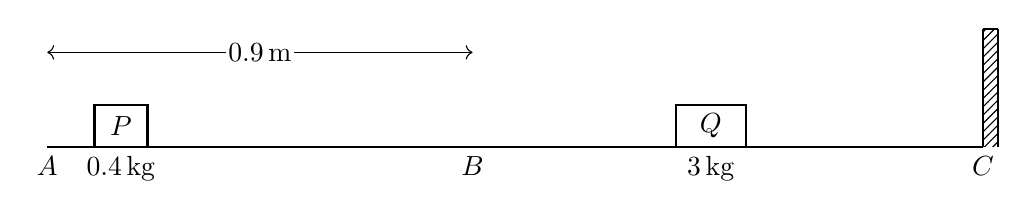
\begin{tikzpicture}[scale=1.2]
\def\AB{4}
\def\BC{5.4}
\def\bwP{0.56}
\def\bwQ{0.74}
\def\bh{0.44}
\def\wallh{1.25}
\def\wallw{0.16}

\coordinate (A) at (-0.5,0);
\coordinate (B) at (\AB,0);
\coordinate (C) at (\AB+\BC,0);

\coordinate (Psw) at ($(A)+(0.5,0)$);
\coordinate (Pne) at ($(Psw)+(\bwP,\bh)$);
\coordinate (Pbr) at ($(Psw)+(\bwP,0)$);

\coordinate (Qsw) at ($(B)+(2.15,0)$);
\coordinate (Qne) at ($(Qsw)+(\bwQ,\bh)$);
\coordinate (Qbr) at ($(Qsw)+(\bwQ,0)$);

\draw[thick] (A) -- (B);
\draw[thick] (B) -- (C);

\draw[<->] ($(A)+(0,1)$) -- node[fill=white, inner sep=1pt] {$0.9\,\mathrm{m}$} ($(B)+(0,1)$);

\draw[thick] (Psw) rectangle (Pne);
\draw[thick] (Qsw) rectangle (Qne);

\node at ($(Psw)!0.5!(Pne)$) {$P$};
\node at ($(Qsw)!0.5!(Qne)$) {$Q$};

\node[below] at ($(Psw)!0.5!(Pbr)$) {$0.4\,\mathrm{kg}$};
\node[below] at ($(Qsw)!0.5!(Qbr)$) {$3\,\mathrm{kg}$};

\fill[pattern=north east lines] (C) rectangle ++(\wallw,\wallh);
\draw[thick] (C) -- ++(0,\wallh);
\draw[thick] ($(C)+(\wallw,0)$) -- ++(0,\wallh);
\draw[thick] ($(C)+(0,\wallh)$) -- ++(\wallw,0);

\node[below] at (A) {$A$};
\node[below] at (B) {$B$};
\node[below] at (C) {$C$};
\end{tikzpicture}
\end{figure}


The diagram shows two blocks $P$ and $Q$ of masses $0.4\,\mathrm{kg}$ and $3\,\mathrm{kg}$ respectively, on a horizontal surface. The points $A$, $B$ and $C$ lie on the surface in a straight line. The surface between $A$ and $B$ is rough and the surface between $B$ and $C$ is smooth. There is a wall at $C$. \\

The coefficient of friction between $P$ and $AB$ is $\dfrac{25}{49}$ \\

Initially, $P$ is at $A$ and $Q$ is at rest on $BC$. Block $P$ is projected directly towards $Q$ with speed $5\,\mathrm{m}\,\mathrm{s}^{-1}$. The two blocks collide on $BC$. As a result of the collision, $P$ changes direction and comes to rest at $A$. You may assume that $P$ only collides with $Q$ once. \\
\begin{enumerate}[label=\textbf{(\alph*)}]
  \item Determine the coefficient of restitution between $P$ and $Q$. \marks{6} \\
  \item Calculate the impulse exerted on $P$ by $Q$ during the collision. \marks{2} \\
\end{enumerate}
After the collision with $P$, block $Q$ strikes the wall at $C$. The collision between $Q$ and the wall is perfectly elastic. After rebounding from the wall, $Q$ comes to rest at a point on $AB$ that is $0.30\,\mathrm{m}$ from $A$. \\
\begin{enumerate}[label=\textbf{(\alph*)}, resume]
  \item Determine the coefficient of friction between $Q$ and $AB$. \marks{3} \\
\end{enumerate}

\newpage

% ---- Question 7 ----
\questionitem
% [Source: _QBT__Collisions_in_1_Dimension, Q7]

Particle $P$ has mass $m$ and particle $Q$ has mass $7m$. \\

The particles are moving in the same direction along the same straight line on a smooth horizontal surface. \\
Particle $P$ collides directly with particle $Q$. \\
Immediately before the collision, the speed of $P$ is $9u$ and the speed of $Q$ is $u$. \\
After the collision, the direction of motion of $P$ is reversed. \\

The coefficient of restitution between $P$ and $Q$ is $e$. \\
\begin{enumerate}[label=\textbf{(\alph*)}]
  \item Find the complete range of possible values of $e$. \marks{7} \\
  \item Given that $e=\dfrac{3}{4}$, find the total kinetic energy lost in the collision between $P$ and $Q$. \marks{4} \\
\end{enumerate}
After the collision, $P$ hits a smooth fixed vertical wall that is perpendicular to the direction of motion of $P$. Particle $P$ rebounds. \\
The coefficient of restitution between $P$ and the wall is $f$. \\

Given that there is a second collision between $P$ and $Q$, \\
\begin{enumerate}[label=\textbf{(\alph*)}, resume]
  \item find the complete range of possible values of $f$. \marks{3} \\
\end{enumerate}

\newpage

% ---- Question 8 ----
\questionitem
% [Source: _QBT__Collisions_in_1_Dimension, Q8]

A particle $A$ of mass $3m$ is moving with speed $4u$ on a smooth horizontal plane towards a smooth fixed vertical wall. A particle $B$ of mass $m$ is on the same line between $A$ and the wall, moving directly towards $A$ with speed $u$. \\

Particles $A$ and $B$ collide directly. The coefficient of restitution between $A$ and $B$ is $e$, where $0<e\le 1$. \\
\begin{enumerate}[label=\textbf{(\alph*)}]
  \item Show that immediately after the collision $B$ moves towards the wall with speed $\dfrac{u}{4}(11+15e)$. \marks{6} \\
  \item Show that there will be a second collision between $A$ and $B$ after $B$ has collided with the wall. \marks{3} \\
\end{enumerate}
The coefficient of restitution between $B$ and the wall is
\(
\dfrac{1}{3}
\) \\

Find, in simplified form, in terms of $m$, $u$ and $e$, \\
\begin{enumerate}[label=\textbf{(\alph*)}, resume]
  \item the magnitude of the impulse received by $B$ from the wall, \marks{3} \\
  \item the loss in kinetic energy of $B$ due to its collision with the wall. \marks{3} \\
\end{enumerate}

\newpage

% ---- Question 9 ----
\questionitem
% [Source: _QBT__Collisions_in_1_Dimension, Q9]

A particle $P$ of mass $m$ is moving in a straight line with speed $5u$ on a smooth horizontal plane. It collides directly with a particle $Q$ of mass $4m$ that is initially at rest on the plane. \\

The coefficient of restitution between $P$ and $Q$ is $e$, where $e>\dfrac{2}{3}$. \\

\begin{enumerate}[label=\textbf{(\alph*)}]
  \item Show that the speed of $P$ immediately after the collision is
  \[
  (4e-1)u
  \]
  \marks[-20pt]{4}
\end{enumerate}
After the collision, $P$ moves in the opposite direction and strikes a smooth fixed vertical wall that is perpendicular to the direction of motion of $P$. The coefficient of restitution between $P$ and the wall is $f$. \\

\begin{enumerate}[label=\textbf{(\alph*)}, resume]
  \item Find, in terms of $e$, the set of values of $f$ for which there will be a second collision between $P$ and $Q$. \marks{6} \\
\end{enumerate}

\newpage

% ---- Question 10 ----
\questionitem
% [Source: _QBT__Collisions_in_1_Dimension, Q10]

\begin{figure}[H]
    \centering
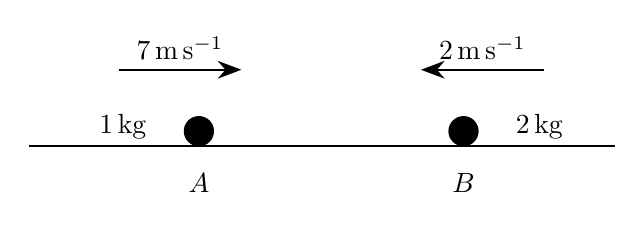
\begin{tikzpicture}[scale=1.2]
\def\rad{0.16}
\coordinate (A) at (1.2,\rad);
\coordinate (B) at (4.0,\rad);
\draw[thick] (-0.6,0) -- (5.6,0);
\fill (A) circle (\rad);
\fill (B) circle (\rad);
\draw[-{Stealth[length=3mm]}, thick] ($(A)+(-0.85,0.65)$) -- ++(1.3,0) node[midway, above] {$7\,\mathrm{m\,s^{-1}}$};
\draw[-{Stealth[length=3mm]}, thick] ($(B)+(0.85,0.65)$) -- ++(-1.3,0) node[midway, above] {$2\,\mathrm{m\,s^{-1}}$};
\node[left] at ($(A)+(-0.45,0.05)$) {$1\,\mathrm{kg}$};
\node[right] at ($(B)+(0.45,0.05)$) {$2\,\mathrm{kg}$};
\node[below] at ($(A)+(0,-0.35)$) {$A$};
\node[below] at ($(B)+(0,-0.35)$) {$B$};
\end{tikzpicture}
\end{figure}


Two small uniform smooth spheres $A$ and $B$ have masses $1\,\mathrm{kg}$ and $2\,\mathrm{kg}$ respectively. The spheres are moving towards each other in the same straight line on a smooth horizontal surface. Sphere $A$ is moving to the right with speed $7\,\mathrm{m\,s^{-1}}$ and sphere $B$ is moving to the left with speed $2\,\mathrm{m\,s^{-1}}$. The spheres collide. After the collision, $A$ moves with speed $1\,\mathrm{m\,s^{-1}}$. \\

Determine the possible speeds with which $B$ moves after the collision. \marks{4}

\newpage

% ---- Question 11 ----
\questionitem
% [Source: _QBT__Collisions_in_1_Dimension, Q11]

Particles $P$ and $Q$, of masses $m$ and $3m$ respectively, move on a smooth horizontal plane in the same straight line towards a vertical wall. Particle $Q$ is in front of $P$. Initially, $P$ has speed $6u$ and $Q$ has speed $u$. Particle $P$ catches up with $Q$ and the particles collide before either particle reaches the wall. \\

The coefficient of restitution between the particles is $e$. \\

As a result of the collision, the direction of motion of $P$ is reversed. \\

\begin{enumerate}[label=\textbf{(\alph*)}]
  \item Find, in terms of $u$ and $e$, the speed of $P$ after the collision. \marks{6} \\
\end{enumerate}
After the collision, $Q$ continues to the wall and rebounds. The coefficient of restitution between $Q$ and the wall is $\dfrac{1}{3}$. \\

Given that there is a second collision between $P$ and $Q$, \\

\begin{enumerate}[label=\textbf{(\alph*)}, resume]
  \item find the full range of possible values of $e$. \marks{5} \\
\end{enumerate}

\newpage

% ---- Question 12 ----
\questionitem
% [Source: _QBT__Collisions_in_1_Dimension, Q12]

Two small uniform smooth spheres $A$ and $B$, of masses $2\,\mathrm{kg}$ and $6\,\mathrm{kg}$ respectively, are on a smooth horizontal surface. Sphere $A$ is projected directly towards $B$ with speed $4\,\mathrm{m}\,\mathrm{s}^{-1}$. Sphere $B$ is initially at rest. The coefficient of restitution between $A$ and $B$ is $e$. \\
\begin{enumerate}[label=\textbf{(\alph*)}]
  \item Show that the velocity of $A$ after the collision, in the original direction of motion of $A$, is $(1-3e)\,\mathrm{m}\,\mathrm{s}^{-1}$ and find a similar expression for the velocity of $B$. \marks{5} \\
  \item The following three parts are independent of each other, and each considers a different scenario regarding the collision between $A$ and $B$. \\
  \begin{enumerate}[label=(\roman*)]
    \item In the collision between $A$ and $B$ the spheres coalesce to form a combined body $C$. State the speed of $C$ after the collision. \marks{1}
    \item In the collision between $A$ and $B$ the direction of motion of $A$ is reversed. Find the range of possible values of $e$. \marks{2}
    \item The total loss in kinetic energy due to the collision is $9\,\mathrm{J}$. Determine the value of $e$. \marks{4} \\
  \end{enumerate}
\end{enumerate}

\end{enumerate}
\end{document}
